\section{Multi-threading}\label{Multi-threading}
The asynchronous part of the A3C algorithm implies a multiplicity of agents trained simultaneously. The different workers share a global network, but train in separate environments. This means that each worker interacts with its own environment, which is a track he is running on. The worker drives the car in a specified track until it crashes, and another frame starts. In such a way, the workers get to explore more of the same track, while incrementally updating a global shared network. This global network is used and continually updated by all the training workers. This facilitates the process of training in a faster tempo because every worker improves the most recent version of the global network.

The global actor-critic network (ACNetwork) is first declared before the workers. Tensorfow has special dedicated methods for enabling multi-threading, which is the Coordinator. The workers are declared and initialized, after which each of them is assigned to a Thread, where they are started to run their own ACNetwork. The multi-threading process is stopped with join() method when all the workers finished their work.

The following figure shows how much faster the training results to be as the number of parallel workers increases. It was chosen to show the performance of accumulating rewards with 1, 4, and  6 workers training in parallel.
\begin{figure}[H]
	\centering
	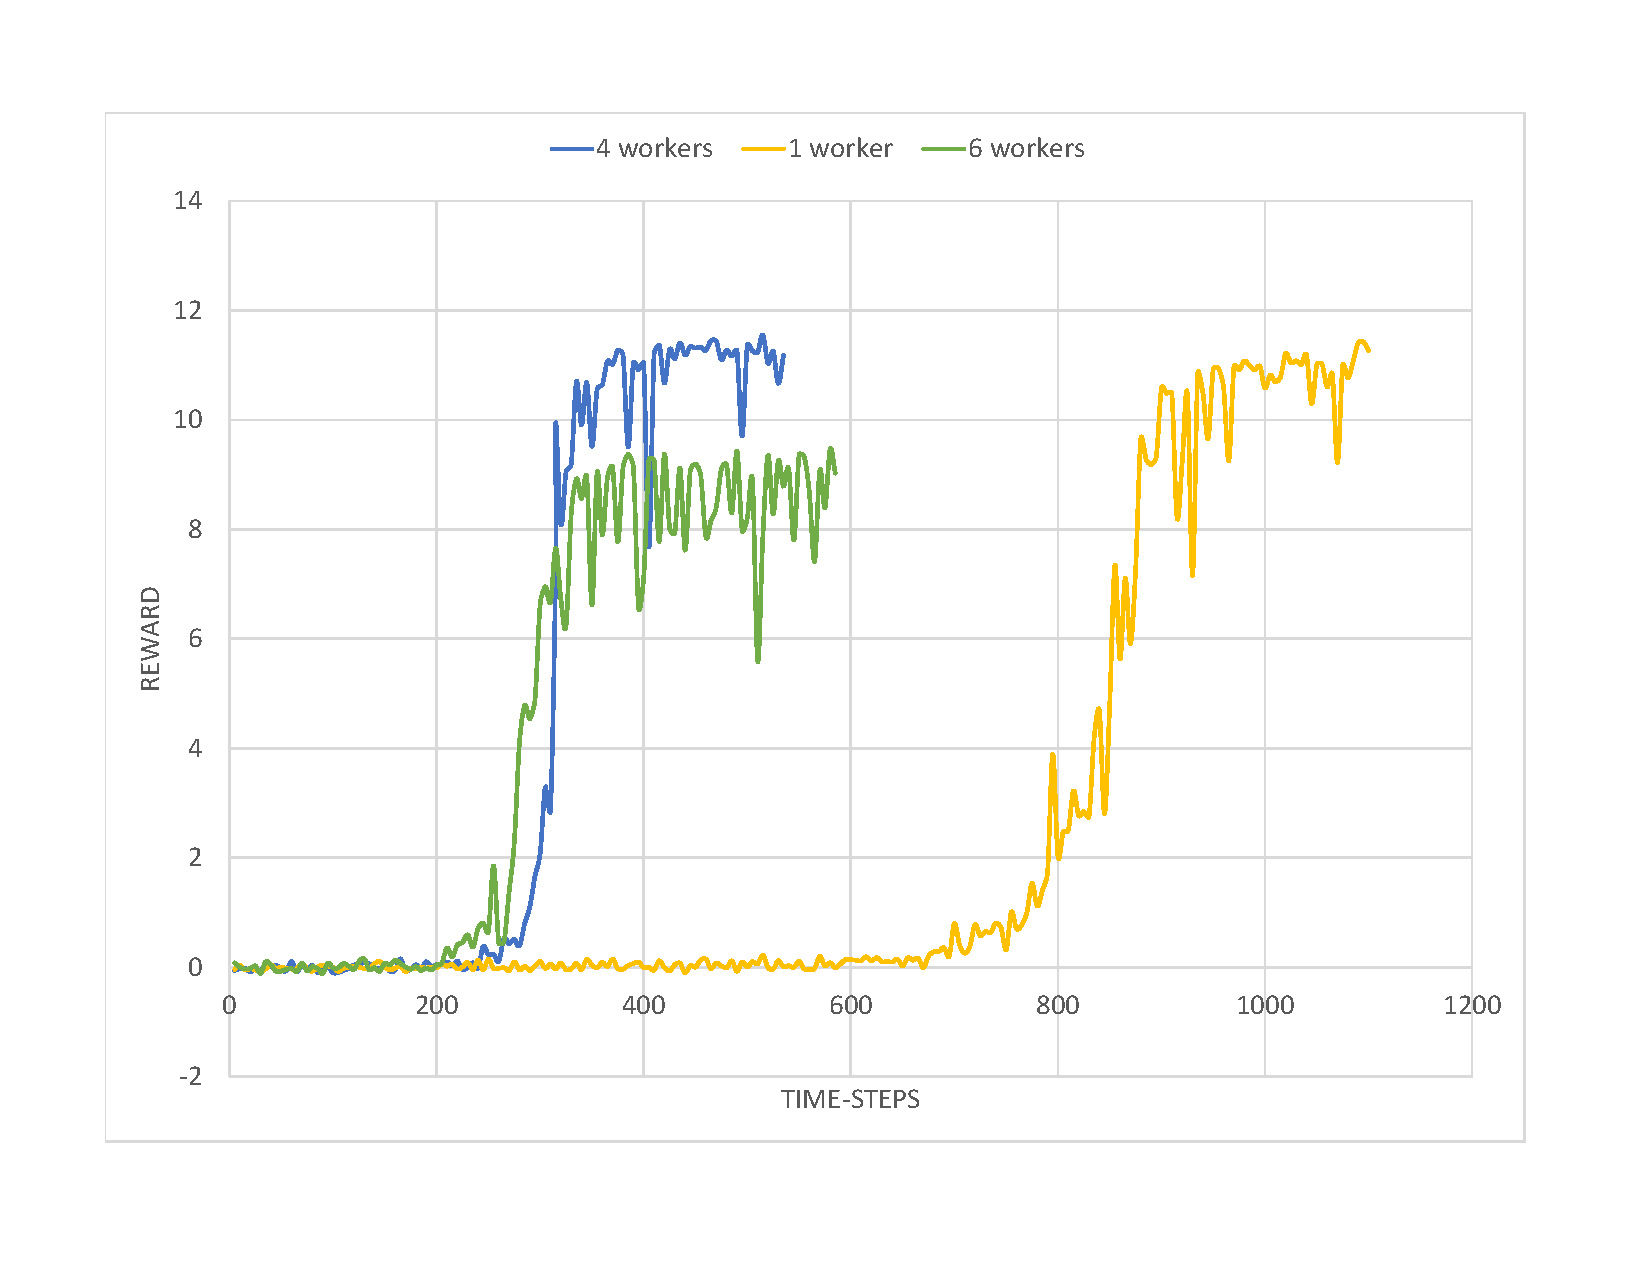
\includegraphics[width=\textwidth]{Figures/Workers}
	\caption{Performance comparison of 1, 4, and 6 workers in parallel}
	\label{fig:Workers}
\end{figure}
 The Figure \ref{fig:Workers} emphasizes that the more workers are used in parallel, the faster the training process becomes. So, for a single worker training alone, the convergence started after 900 time-steps. For 4 workers - the reward function started to grow fast after 250 time-steps, resulting in convergence after 300 time-steps. By increasing the number of workers from 1 to 4, the training became 3 times faster.
 
 It is also possible to see that the training with 6 workers converged to a lower accumulated reward than those of 1 and 4 workers. This is possibly due to a problem of multi-threading the TORCS environment. There are some "Time-out" problems when increasing the number of workers and the performance of the 6 workers was probably affected by it.